\title{Linear Dithering}
%RUN_VERBATIMS sh &

Consider the problem of converting a gray-scale image into a binary image,
while keeping as much as possible of the visual information.
The two standard techniques are {\bf thresholding} and {\bf dithering}.

The goal of this note is to show that thresholding and dithering are just two
points on a multidimensional continuum of binarization methods, that we call
{\bf linear dithering}.

%SCRIPT plambda i/weiro.png "87 > 255 *" -o weiro-bin.png
%SCRIPT dither i/weiro.png weiro-dit.png
%SCRIPT plambda i/weiro.png x,l|blur -z z 0.1|plambda - '0 < 255 *' -o weiro-lin.png
\begin{tabular}{llll}
	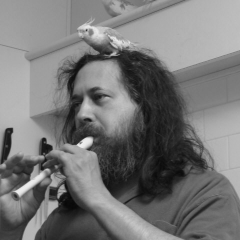
\includegraphics{i/weiro.png} &
	
\includegraphics{weiro-bin.png} &
	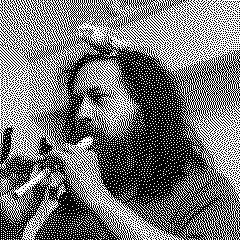
\includegraphics{weiro-dit.png} &
	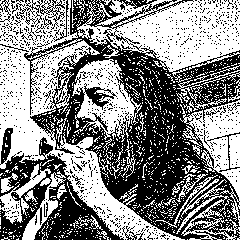
\includegraphics{weiro-z01.png} \\
	original image &
	thresholding &
	dithering &
	linear dithering
\end{tabular}

\section{Classic thresholding and dithering}

Thresholding at the right level is surprisingly effective.  It is often
possible to find a threshold that captures most of the relevant information
in the image, even in the case of extreme lighting conditions.
Yet, it is clear than for some images it will be impossible to find a single
satisfactory threshold.
Dithering (also called error diffusion) is aimed at representing all the
possible gray levels of the original image, at the price of a small loss of
resolution.

Look at this photo of a famous bongo player, for example.  There is a strong
spot light righto into his face, and the rest of the image is very dark.  I
would say that it is impossible to find a single threshold where the face
and the hand are recognizable.  Yet there is!  And quite easy to find
manually, around the value of 87, for example.
We show also the results of Floyd-Sternberg dithering and the linear
dithering described below.  Notice that Floyd-Sternberg dithering destroys
all the texture of the clothes, which is well-preserved by thresholding and
linear dithering.  (Too well-preserved, in the last case, as it enhances the
jpeg compression artifacts of the original.)


\begin{gallery}
	\galleryline{i/bongos.jpg}
	\galleryline{bongos-bin.png}
	\galleryline{bongos-dit.png}
	\galleryline{bongos-lin.png}
\end{gallery}
\begin{verbatim}
plambda i/bongos.jpg "87 > 255 *" -o bongos-bin.png
dither i/bongos.jpg bongos-dit.png
plambda i/bongos.jpg x,l | blur z 0.25 | plambda - '0 < 255 *' -o bongos-lin.png
\end{verbatim}

%\begin{gallery}
%	\galleryline{i/cockatiels.png}
%	\galleryline{cockatiels-bin.png}
%	\galleryline{cockatiels-dit.png}
%\end{gallery}
%\begin{verbatim}
%plambda i/cockatiels.png "87 > 255 *" -o cockatiels-bin.png
%dither i/cockatiels.png cockatiels-dit.png
%\end{verbatim}

\section{Dithering with pre-processing}

We can pre-process gray-scale images before dithering them.  We consider two
pre-processings: a {\bf contrast change} by a function of the
form~$x\mapsto\tanh(\lambda x)/\tanh(\lambda)$, and a {\bf linear filtering}
of the original image that enhances its contrast.  For simplicity, here we
assume that our input images are of zero mean and take values on~$[-1,1]$.

For the contrast change, notice two things.  First, the
$\lambda$-scaled~$\tanh$ tends to a step function as~$\lambda\to\infty$, and
to the identity on~$[-1,1]$ as~$\lambda\to0$.
Second, dithering a binary image produces exactly the same image.  Thus, just
by composing the dithering with a contrast change, we obtain a one-parameter
family of methods that contains pure dithering and pure
binarization as particular cases.

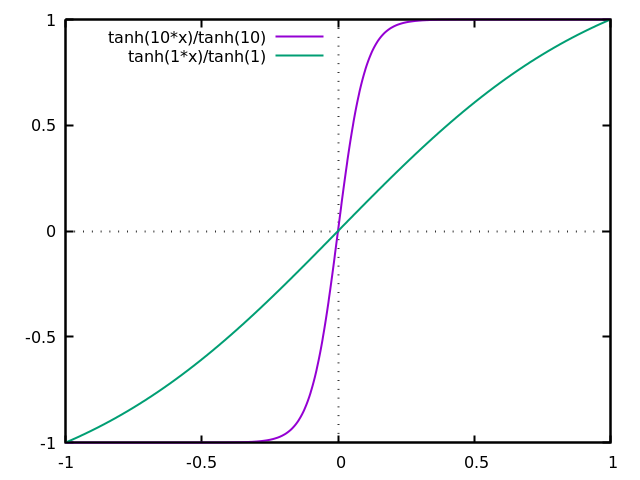
\includegraphics{tanhs.png}
%SCRIPT gnuplot <<END >tanhs.png
%SCRIPT set term pngcairo lw 2
%SCRIPT set samples 1000
%SCRIPT set zeroaxis
%SCRIPT set key top left
%SCRIPT plot [-1:1] [-1:1] tanh(10*x)/tanh(10),tanh(1*x)/tanh(1)
%SCRIPT END


In the figures below, the first row contains the result of applying the
contrast change, and the second row the dithering of each image.

%SCRIPT ditanh() { plambda "127 - 127 / $1 * tanh $1 tanh / 127 * 127 +" ; }
%SCRIPT cat i/weiro.png | ditanh 0.1 | iion - weiro-tanh0.png
%SCRIPT cat i/weiro.png | ditanh 3   | iion - weiro-tanh3.png
%SCRIPT cat i/weiro.png | ditanh 7   | iion - weiro-tanh7.png
%SCRIPT cat i/weiro.png | ditanh 900 | iion - weiro-tanhi.png
%SCRIPT cat i/weiro.png | ditanh 0.1 | dither - weiro-ditanh0.png
%SCRIPT cat i/weiro.png | ditanh 3   | dither - weiro-ditanh3.png
%SCRIPT cat i/weiro.png | ditanh 7   | dither - weiro-ditanh7.png
%SCRIPT cat i/weiro.png | ditanh 900 | dither - weiro-ditanhi.png
\begin{tabular}{llll}
	$\lambda=0$ &
	$\lambda=3$ &
	$\lambda=7$ &
	$\lambda=\infty$ \\
	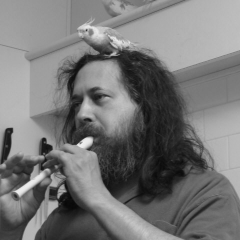
\includegraphics{weiro-tanh0.png} &
	
\includegraphics{weiro-tanh3.png} &
	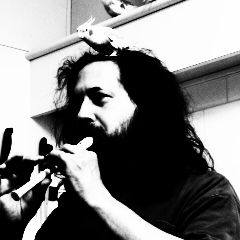
\includegraphics{weiro-tanh7.png} &
	
\includegraphics{weiro-tanhi.png} \\
	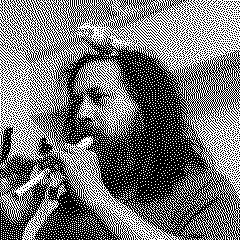
\includegraphics{weiro-ditanh0.png} &
	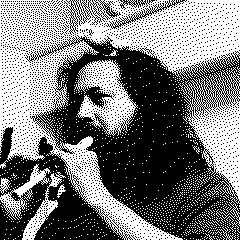
\includegraphics{weiro-ditanh3.png} &
	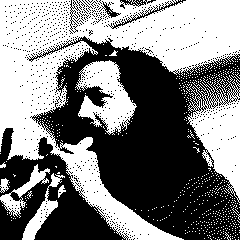
\includegraphics{weiro-ditanh7.png} &
	
\includegraphics{weiro-ditanhi.png} \\
\end{tabular}

For the linear filtering, we consider a family of filters~$k$ of the
form~$\widehat{k}(\xi)=|\xi|^\mu$ for~$\mu\in[0,2]$, acting over images of
zero mean, suitably normalized to conserve the second moment of the image.
These filters interpolate continuously between the identity ($\mu=0$) and
minus the Laplacian operator ($\mu=2$).  The case~$\mu=1$ can be
called~\emph{linear retinex}.  For~$\mu<0$, this is called the Riesz scale
space.


%SCRIPT riesz() { periodize | fft | plambda ":R $1 ^ *" | ifft | imhalve ; }
%SCRIPT cat i/weiro.png | riesz 0.1 | qauto - weiro-riesz01.png            &
%SCRIPT cat i/weiro.png | riesz 0.5 | qauto - weiro-riesz05.png            &
%SCRIPT cat i/weiro.png | riesz 1.0 | qauto - weiro-riesz10.png            &
%SCRIPT cat i/weiro.png | riesz 2.0 | qauto - weiro-riesz20.png            &
%SCRIPT cat i/weiro.png | riesz 0.1 | qauto | dither - weiro-diriesz01.png &
%SCRIPT cat i/weiro.png | riesz 0.5 | qauto | dither - weiro-diriesz05.png &
%SCRIPT cat i/weiro.png | riesz 1.0 | qauto | dither - weiro-diriesz10.png &
%SCRIPT cat i/weiro.png | riesz 2.0 | qauto | dither - weiro-diriesz20.png &
%SCRIPT wait
\begin{tabular}{llll}
	$\mu=0.1$ &
	$\mu=0.5$ &
	$\mu=1$ &
	$\mu=2$\\
	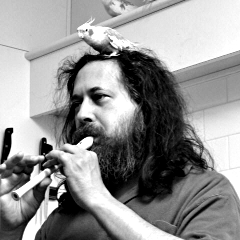
\includegraphics{weiro-riesz01.png} &
	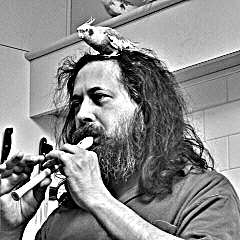
\includegraphics{weiro-riesz05.png} &
	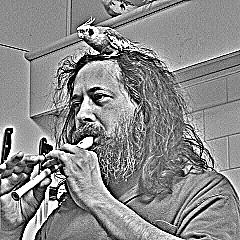
\includegraphics{weiro-riesz10.png} &
	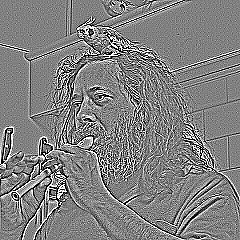
\includegraphics{weiro-riesz20.png} \\
	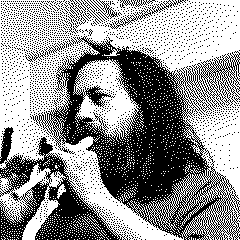
\includegraphics{weiro-diriesz01.png} &
	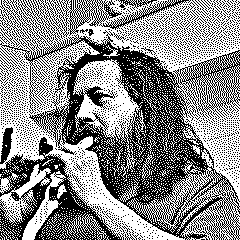
\includegraphics{weiro-diriesz05.png} &
	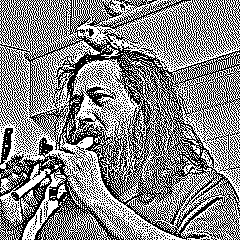
\includegraphics{weiro-diriesz10.png} &
	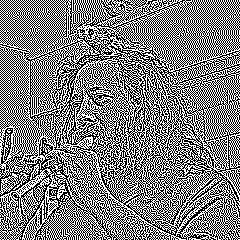
\includegraphics{weiro-diriesz20.png} \\
\end{tabular}

Notice that the Laplacian is locally constant nearly everywhere, except just
around the edges.  Thus, dithering this image results in a checkerboard
pattern of density $50\%$, but with a characteristic bias around the edges
which renders the structures visible.


\section{Thresholding with linear pre-processing}

Now, forget a moment about the dithering step and consider only linear
filtering and thresholding.
In modern parlance, thresholding with linear pre-processing would be called
\emph{single layer convolutional neural network with Heaviside activation
function}.

More precisely, we take an image of zero mean, apply a linear filter, and
threshold the result at 0.


Let us see how changing shape of the kernel produces
different effects.  We use the following radial kernels (we omit the
normalization factors in this table):
\begin{tabular}{ll}
	name & formula \\
	Gauss & $G_\sigma(r) =\delta-\exp\frac{-r^2}{2\sigma^2}$ \\
	Laplace & $L_\sigma(r) =\delta-\exp\frac{-r}{\sigma}$ \\
	Cauchy & $C_\sigma(r) =\delta-\frac{1}{\sigma^2+r^2}$ \\
	Riesz & $\widehat{R_\sigma}(\rho)=\rho^\sigma$ \\
	truncated inverse-log & $Z_\sigma(r)=T_\sigma\frac{1}{\log(r)}$\\
	log-Cauchy & $Q_\sigma(r)=-\log(\sigma^2+r^2)$ \\
\end{tabular}

These filters are all positive, so the effect they produce is blurring the
images.  For this application we apply them to the Laplacian of the input
image (or, equivalently, we filter the image by the Laplacian of these
kernels).

%%SCRIPT blur -s G  1 i/weiro.png|plambda - '0 > 255 *' -o weiro-G01.png
%%SCRIPT blur -s G  5 i/weiro.png|plambda - '0 > 255 *' -o weiro-G05.png
%%SCRIPT blur -s G 15 i/weiro.png|plambda - '0 > 255 *' -o weiro-G15.png
%\begin{tabular}{lll}
%	\includegraphics{weiro-G01.png} &
%	\includegraphics{weiro-G05.png} &
%	\includegraphics{weiro-G15.png} \\
%	$G_{1}$ &
%	$G_{5}$ &
%	$G_{15}$ \\
%\end{tabular}
%
%%SCRIPT blur -s L  1 i/weiro.png|plambda - '0 > 255 *' -o weiro-L01.png
%%SCRIPT blur -s L  5 i/weiro.png|plambda - '0 > 255 *' -o weiro-L05.png
%%SCRIPT blur -s L 15 i/weiro.png|plambda - '0 > 255 *' -o weiro-L15.png
%\begin{tabular}{lll}
%	\includegraphics{weiro-L01.png} &
%	\includegraphics{weiro-L05.png} &
%	\includegraphics{weiro-L15.png} \\
%	$L_{1}$ &
%	$L_{5}$ &
%	$L_{15}$ \\
%\end{tabular}
%
%%SCRIPT blur -s C 1e-3 i/weiro.png|plambda - '0 > 255 *' -o weiro-C01.png
%%SCRIPT blur -s C  1 i/weiro.png|plambda - '0 > 255 *' -o weiro-C05.png
%%SCRIPT blur -s C 1e5 i/weiro.png|plambda - '0 > 255 *' -o weiro-C15.png
%\begin{tabular}{lll}
%	\includegraphics{weiro-C01.png} &
%	\includegraphics{weiro-C05.png} &
%	\includegraphics{weiro-C15.png} \\
%	$C_{1}$ &
%	$C_{5}$ &
%	$C_{15}$ \\
%\end{tabular}

%SCRIPT plambda x,l<i/weiro.png|blur -z g 0.5|plambda - '0 < 255 *' -o weiro-ga.png
%SCRIPT plambda x,l<i/weiro.png|blur -z g 1|plambda - '0 < 255 *' -o weiro-gb.png
%SCRIPT plambda x,l<i/weiro.png|blur -z g 3|plambda - '0 < 255 *' -o weiro-gc.png
\begin{tabular}{lll}
	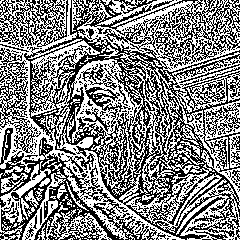
\includegraphics{weiro-ga.png} &
	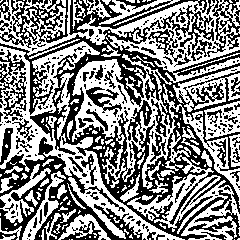
\includegraphics{weiro-gb.png} &
	
\includegraphics{weiro-gc.png} \\
	$G_{0.5}$ &
	$G_{1}$ &
	$G_{3}$ \\
\end{tabular}

%SCRIPT plambda x,l<i/weiro.png|blur -z l 0.5|plambda - '0 < 255 *' -o weiro-la.png
%SCRIPT plambda x,l<i/weiro.png|blur -z l 1|plambda - '0 < 255 *' -o weiro-lb.png
%SCRIPT plambda x,l<i/weiro.png|blur -z l 3|plambda - '0 < 255 *' -o weiro-lc.png
\begin{tabular}{lll}
	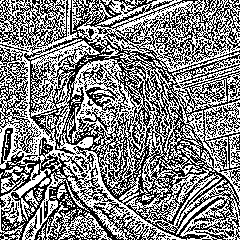
\includegraphics{weiro-la.png} &
	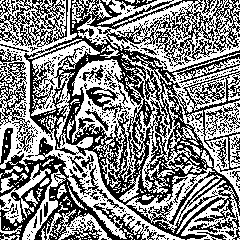
\includegraphics{weiro-lb.png} &
	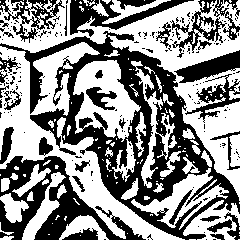
\includegraphics{weiro-lc.png} \\
	$L_{0.5}$ &
	$L_{1}$ &
	$L_{3}$ \\
\end{tabular}

%SCRIPT plambda x,l<i/weiro.png|blur -z c 0.5|plambda - '0 < 255 *' -o weiro-ca.png
%SCRIPT plambda x,l<i/weiro.png|blur -z c 1|plambda - '0 < 255 *' -o weiro-cb.png
%SCRIPT plambda x,l<i/weiro.png|blur -z c 3|plambda - '0 < 255 *' -o weiro-cc.png
\begin{tabular}{lll}
	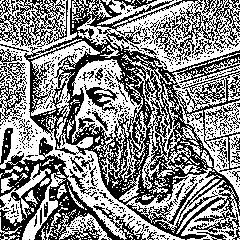
\includegraphics{weiro-ca.png} &
	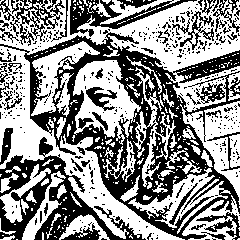
\includegraphics{weiro-cb.png} &
	
\includegraphics{weiro-cc.png} \\
	$C_{0.5}$ &
	$C_{1}$ &
	$C_{3}$ \\
\end{tabular}

%SCRIPT plambda i/weiro.png x,l|blur -z z 0.01|plambda - '0 < 255 *' -o weiro-z01.png
%SCRIPT plambda i/weiro.png x,l|blur -z z 0.10|plambda - '0 < 255 *' -o weiro-z10.png
%SCRIPT plambda i/weiro.png x,l|blur -z z 0.20|plambda - '0 < 255 *' -o weiro-z20.png
%SCRIPT plambda i/weiro.png x,l|blur -z z 0.50|plambda - '0 < 255 *' -o weiro-z50.png
\begin{tabular}{llll}
	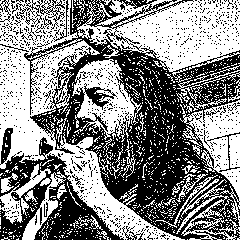
\includegraphics{weiro-z01.png} &
	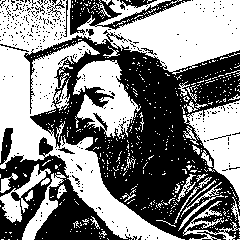
\includegraphics{weiro-z10.png} &
	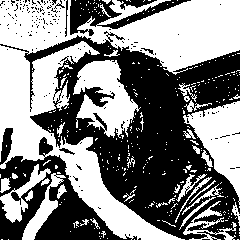
\includegraphics{weiro-z20.png} &
	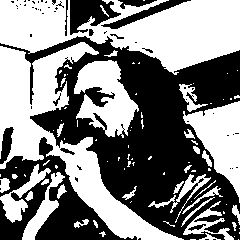
\includegraphics{weiro-z50.png} \\
	$Z_{0.01}$ &
	$Z_{0.10}$ &
	$Z_{0.20}$ &
	$Z_{0.50}$
\end{tabular}

%SCRIPT plambda i/weiro.png x,l|blur -z i 0.01|plambda - '0 < 255 *' -o weiro-i01.png
%SCRIPT plambda i/weiro.png x,l|blur -z i 0.10|plambda - '0 < 255 *' -o weiro-i10.png
%SCRIPT plambda i/weiro.png x,l|blur -z i 0.20|plambda - '0 < 255 *' -o weiro-i20.png
%SCRIPT plambda i/weiro.png x,l|blur -z i 0.50|plambda - '0 < 255 *' -o weiro-i50.png
\begin{tabular}{llll}
	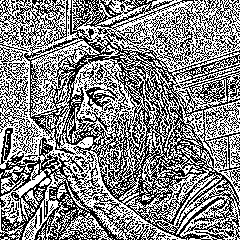
\includegraphics{weiro-i01.png} &
	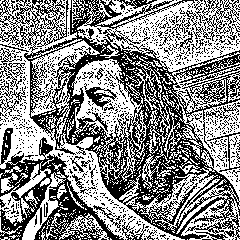
\includegraphics{weiro-i10.png} &
	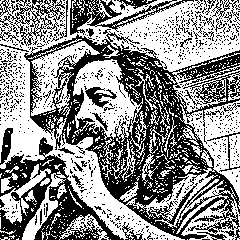
\includegraphics{weiro-i20.png} &
	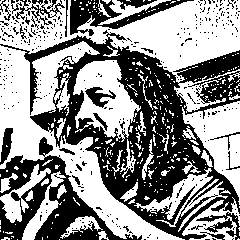
\includegraphics{weiro-i50.png} \\
	$Y_{0.01}$ &
	$Y_{0.10}$ &
	$Y_{0.20}$ &
	$Y_{0.50}$
\end{tabular}

%SCRIPT plambda i/weiro.png x,l|blur -z q 0.01|plambda - '0 < 255 *' -o weiro-q01.png
%SCRIPT plambda i/weiro.png x,l|blur -z q 0.10|plambda - '0 < 255 *' -o weiro-q10.png
%SCRIPT plambda i/weiro.png x,l|blur -z q 0.20|plambda - '0 < 255 *' -o weiro-q20.png
%SCRIPT plambda i/weiro.png x,l|blur -z q 0.50|plambda - '0 < 255 *' -o weiro-q50.png
\begin{tabular}{llll}
	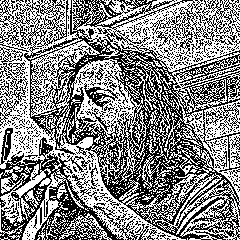
\includegraphics{weiro-q01.png} &
	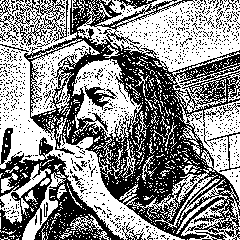
\includegraphics{weiro-q10.png} &
	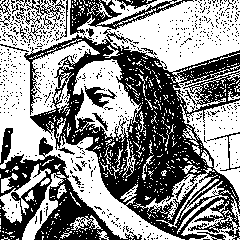
\includegraphics{weiro-q20.png} &
	\includegraphics{weiro-q50.png} \\
	$Q_{0.01}$ &
	$Q_{0.10}$ &
	$Q_{0.20}$ &
	$Q_{0.50}$
\end{tabular}

Notice that some of these images (e.g.,~$Y_{20}$ and~$Q_{20}$) could pass ass
``dithering'', but with sharper edges.  However, they are simply a
thresholding of the image after a linear filter, where the kernel has been
chosen carefully.

This is just a small exploration of a huge family of {\bf linear dithering}
methods to produce binary images, that contains thresholding and dithering by
error diffusion as
particular cases.

This technique also works for color images, by treating each RGB channel
independently, and producing a 3-bit palette at the end.  Compared to
traditional dithering error diffusion, it allows a much higher resolution, at
the price of a considerable loss in color fidelity, due to saturation.
However, the saturation is much less than for a brutal per-channel
binarization.   See, for example, the
blue eyes in this color image:

\begin{verbatim}
dither i/barb.png barb-dit.png
plambda i/barb.png x,l | blur z 0.15 | plambda - '0 < 255 *' -o barb-lin.png
plambda i/barb.png 'x x%O50 > 255 *' -o barb-bin.png
\end{verbatim}
\begin{gallery}
	\galleryline{i/barb.png}
	\galleryline{barb-dit.png}
	\galleryline{barb-lin.png}
	\galleryline{barb-bin.png}
\end{gallery}


\small
PS: all the experiments on this note are generated from comments extracted
of the original .tex source file.


%\section{Two-layer binarization}

% vim:set tw=77 filetype=tex spell spelllang=en:
